\documentclass{article} % For LaTeX2e
\usepackage{nips15submit_e,times}
\usepackage{hyperref}
\usepackage{url}
\usepackage{amssymb,amsmath}
\usepackage[pdftex]{graphicx}
%\documentstyle[nips14submit_09,times,art10]{article} % For LaTeX 2.09


\title{Variational Bayesian Inference for Neural Feature Tagging in Unstructured Stimuli}


\author{
John M.~Pearson\\
Duke Institute for Brain Sciences \\
Duke University\\
Durham, NC 27708 \\
\texttt{john.pearson@duke.edu} \\
\And
Jeffrey M.~Beck \\
Department of Neurobiology \\
Duke University Medical Center \\
Durham, NC 27708 \\
\texttt{jeff.beck@duke.edu} \\
}

% The \author macro works with any number of authors. There are two commands
% used to separate the names and addresses of multiple authors: \And and \AND.
%
% Using \And between authors leaves it to \LaTeX{} to determine where to break
% the lines. Using \AND forces a linebreak at that point. So, if \LaTeX{}
% puts 3 of 4 authors names on the first line, and the last on the second
% line, try using \AND instead of \And before the third author name.

\newcommand{\fix}{\marginpar{FIX}}
\newcommand{\new}{\marginpar{NEW}}

% \nipsfinalcopy % Uncomment for camera-ready version

\begin{document}


\maketitle

\begin{abstract}
Typically, experiments studying stimulus encoding at the level of individual neurons choose a small set of features present in the world --- contrast and luminance for vision, pitch and intensity for sound --- and assemble a set of stimuli that systematically varies along these dimensions. Neuronal responses in the form of firing rates are then tested for systematic variation with respect to these features. However, such an approach requires that experimenters know (or guess) in advance the relevant features coded by a given neural population. For instance, the feature space for socially relevant stimuli is poorly understood, and the need for an \emph{a priori} choice of features may give rise to confirmation bias. Here we present an approach to automatic feature inference in unstructured stimulus sets based on population neuronal responses. Utilizing a Variational Bayesian approach, we construct a model of latent discrete time-varying features with (semi-)Markov dynamics under a Poisson observation model. Our model correctly recovers hidden features in synthetic data as well as ground-truth stimulus features in a prototypical neural dataset. Finally, we apply our method to the problem of feature tagging in a database of naturalistic stimuli based on neural responses in prefrontal cortex.
\end{abstract}

\section{Introduction}
The question of how the brain encodes information from the natural world forms one of the primary areas of study within neuroscience. For many sensory systems, particularly vision and audition, the discovery that single neurons modulate their firing of action potentials in response to particular stimulus features has proven foundational for theories of sensory function. Indeed, neuronal responses to contrast, edges, and motion direction appear to form fundamental primitives on which higher-level visual abstractions are built. Nevertheless, many of these higher-level abstractions, increasingly of interested to modern neuroscience, do not exist in a stimulus space with obvious axes. As a result, experimentalists must choose \emph{a priori} features of interest in constructing their stimulus sets, with the result that cells may appear broadly and weakly tuned due to misalignment of stimulus and neural axes.

In vision, methods like reverse correlation have proven successful in elucidating response properties of some cell types, but such techniques rely on a well-behaved stimulus space and a highly constrained encoding model in order to achieve sufficient statistical power to perform inference \cite{steveninck1988realtime,ringach2004reverse,ringach2002receptive}. However, natural stimuli are known to violate both criteria, and generate patterns of neural activity that differ markedly from those observed in controlled experiments with limited stimulus complexity \cite{ringach2002receptive,sharpee2004analyzing,Vinje2000-dx}. Information-based approaches have gone some way in addressing this challenge \cite{sharpee2004analyzing}, but this approach must often assume a metric structure on stimuli in order to optimize encoded information.

More recently, Gallant and collaborators have tackled this problem in the context of fMRI, demonstrating that information present in the blood oxygen level-dependent (BOLD) signal is sufficient to classify and map the representation of natural movie stimuli across the brain \cite{Kay2008-gd,Vu2011-da,Huth2012-cj,Stansbury2013-nm}. These studies have used a number of modeling frameworks, from latent dirichlet allocation for categorizing scene contents \cite{Stansbury2013-nm} to regularized linear regression \cite{Huth2012-cj} to sparse nonparametric models \cite{Vu2011-da} to characterize brain encoding of stimuli, but in each case, models were built on pre-labeled training data. Clearly, a method that could infer stimulus structure from neural data themselves would be able to extend such work to include less easily characterized stimulus sets like those depicting social interaction.

Another recent line of work, this one focused on cascaded linear-nonlinear-Poisson (NLP) models, has addressed itself to the task of modeling dynamics of neural populations at the single unit scale \cite{Pillow2008-em,Vogelstein2009-ax,Park2014-el,Buesing2014-ta}. Using generalized linear models as building blocks, these models have proven able to infer (functional) connectivity \cite{Pillow2008-em}, deconvolve spike times generating a calcium image \cite{Vogelstein2009-ax}, and finding subgroups of responsive neurons \cite{Buesing2014-ta}. Inference is generally performed via expectation maximization, though these models are also closely related to those based on information maximization \cite{Williamson2013-rg}.

Our model sits at the intersection of these two approaches. We use Variational Bayesian methods, closely related to expectation maximization, to perform inference in a framework reminiscent of generalized linear models. We do this to infer latent, time-varying, discrete features in stimulus sets, in our case from observations of spike counts from neural populations. Unlike previous work, we do not assume these features in advance, though our model does allow experimental features of interest to be specified as regressors. In addition, we include a sparse hierarchical prior over individual units' response strengths to each feature, resulting in a parsimonious explanation of firing rates.In this way, our work shares features with that of \cite{Ulrich2014-zc}, which used spectral content of local field potentials (LFP) to classify moment-by-moment neural activity into distinct brain states. Our model differs in two key ways from that approach: (1) our observations are count data (spike counts) as opposed to continuously measured LFPs and (2) our model infers multiple features, each with distinct dynamics, rather than a single class label at each time. Moreover, because most updates in our model utilize conjugate distributions, inference is fast. Finally, our model allows for semi-Markov dynamics in the latent feature space, accommodating features at multiple, distinct time scales.

\section{Model}
\begin{figure}[ht]
    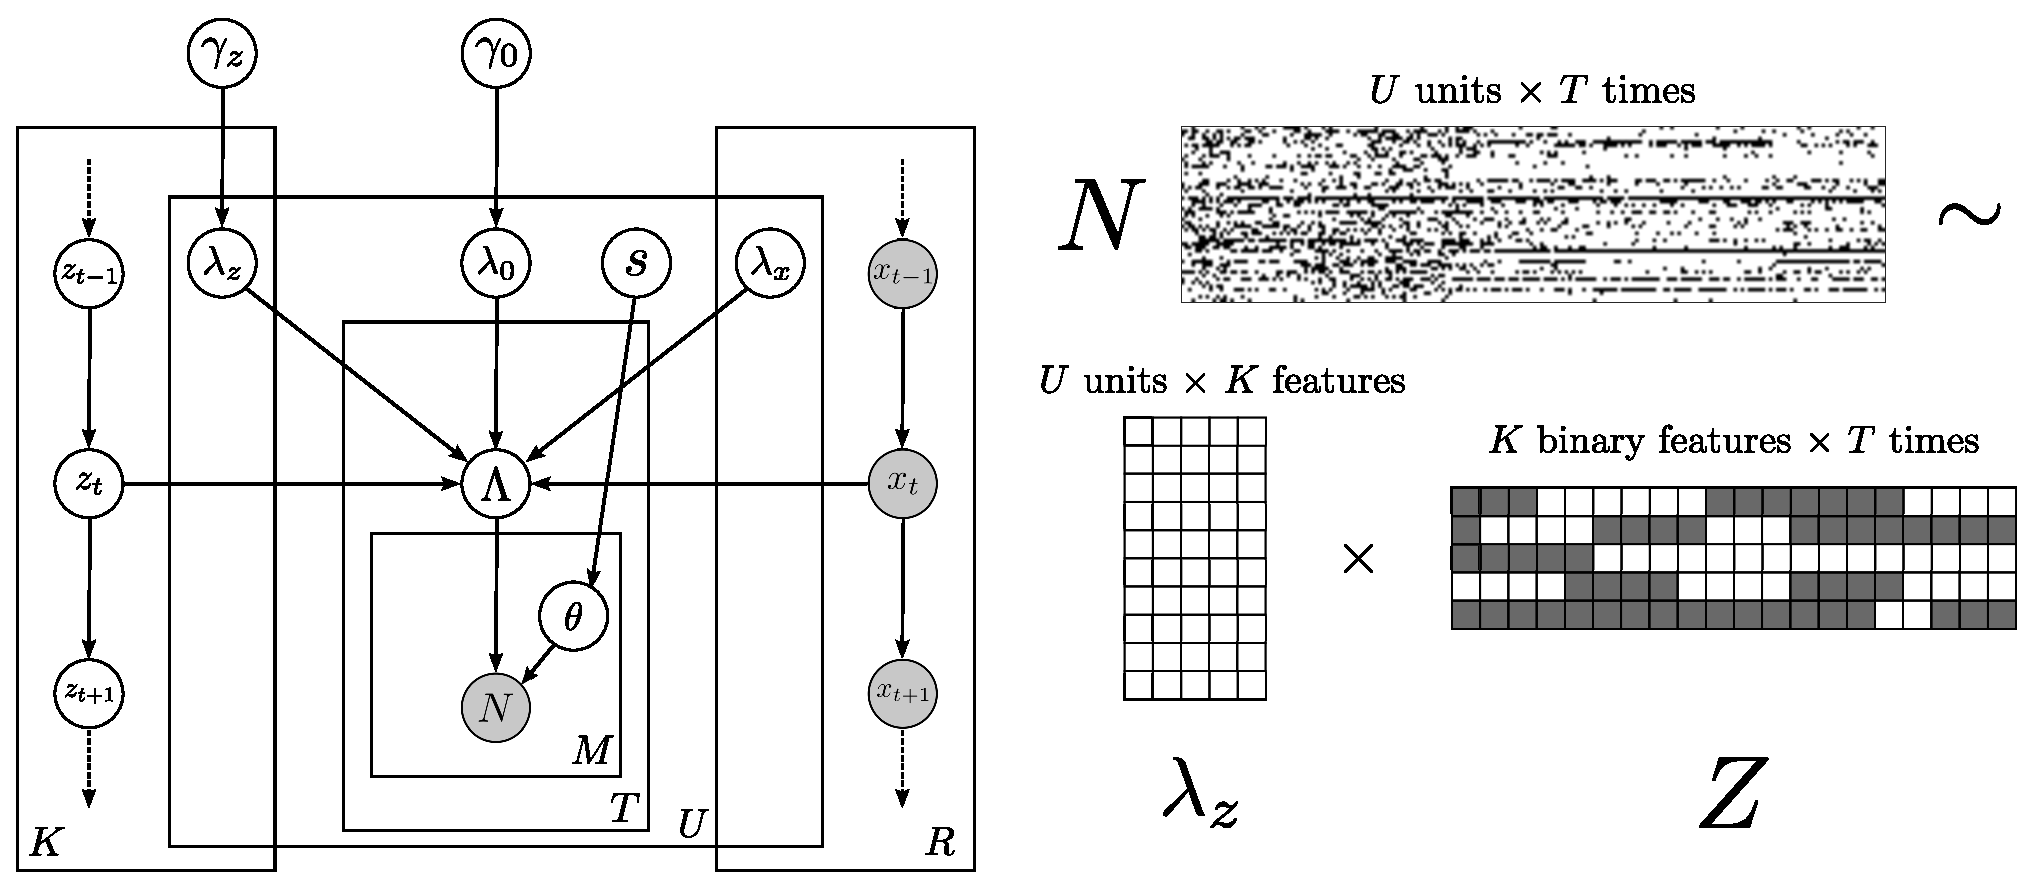
\includegraphics[width=1\linewidth]{figures/model}
    \caption{\textbf{Generative model for spike counts.} Spike counts $N$ are observed for each of $U$ units over stimulus time $T$ for multiple presentations $M$. Counts are assumed Poisson-distributed, with firing rates $\Lambda$ that depend on each unit's responses ($\lambda$) to both latent discrete states $z_t$ and observed regressors $x_t$ that change in time, as well as a baseline firing rate $\lambda_0$. $\gamma$ nodes represent hyperparameters for the firing rate effects. $\theta$ is a multiplicative overdispersion term specific to each observation, distributed according to hyperparameters $s$.}
\end{figure}
\subsection{Observation model}
Consider a population of $U$ spiking neurons exposed to a series of stimuli indexed by a (unique) time index $t\in \lbrace 1\ldots T\rbrace$. Moreover, each neuron is exposed to each stimulus $M_{tu}$ times, where we do not assume either that each neuron observes each stimulus time or that consecutive times are observed by the same sets of neurons. That is $M_{tu}$ may have many 0s. For each observation $m$ (a unique unit, time pair), we then observe a spike count, $N_m$. We model these spike counts as arising from a Poisson process with time-dependent rate $\Lambda_{tu}$ and observation-specific multiplicative overdispersion $\theta_m$:
\begin{align}
    N_{m} &\sim \text{Pois}(\Lambda_{t(m), u(m)} \theta_m) &
    \theta_m &\sim \text{Ga}(s_{u(m)}, s_{u(m)})
\end{align}
Note that both the unit and time are functions of the observation index, $m$, and that the distribution of the overdispersion for each observation is specific to the unit observed. 

\subsection{Firing rate model}
At each stimulus time $t$, we assume the existence of $K$ binary latent states $z_{tk}$ and $R$ observed, continuous regressors $x_{tr}$. We further assume that each unit's firing rate response at each time can be modeled as arising from the product of three effects: (1) a baseline firing rate specific to each unit, (2) a product of responses to each latent state, and (3) a product of responses to each observed regressor:
\begin{equation}
    \Lambda_{tu} = \lambda_{0u} \prod_{k = 1}^K \lambda_{zuk}^{z_{tk}}  
    \prod_{r = 1}^R \lambda_{xur}^{x_{tr}}   
\end{equation} 
Note that this is conceptually similar to the generalized linear model for firing rates (in which we model $\log \Lambda$) with the identification $\beta = \log \lambda$. However, by modeling the firing rate directly as a product and placing Gamma priors on the individual effects, we will be able to take advantage of closed-form variational updates resulting from conjugacy that avoid explicit optimization in the case of the $z$s (see below). 

In addition, to enforce parsimony in the inferred features, we put sparse hierarchical priors on the $\lambda_z$ terms:
\begin{align}
    \lambda_{uk} &\sim \text{Ga}(c_k, c_k d_k) & c_k &\sim \text{Ga}(s_k, r_k)
    & d_k &\sim \text{Ga}(t_k, w_k)
\end{align}
That is, $\mathbb{E}[\lambda_u] = d^{-1}$ and $\text{var}[\lambda_u] = (cd^2)^{-1}$, so for $c$ large and $d\sim \mathcal{O}(1)$, the prior for firing rate response to each latent feature will be strongly concentrated around 0. And once again, this choice of priors will lead to closed-form updates in our variational approximation. Finally, for the baseline terms, $\lambda_{0u}$, we use a non-sparse version of the same model, while for the specified regressor responses, $\lambda_{xu}$, we model the unit effects non-hierarchially using independent Gamma priors for each unit.

\subsection{Latent state model}
We model the latent states $z_{tk}$ as an independent Hidden Markov Model (HMM) for each feature $k$. That is, each $k$ indexes an independent Markov chain with initial state probability $\pi^{(k)}$ and transition matrix $A^{(k)}$. For the semi-Markov case, we assume that the dwell times in each state are distributed independently for each chain according to an integer-valued, truncated lognormal distribution with maximum duration $D$:
\begin{align}
    p_k(d|z = j) &= \text{Log-Normal}(d|m_{kj}, s^2_{kj}) / W  &
    W &= \sum_{d = 1}^D \text{Log-Normal}(d|m_{kj}, s^2_{kj}) 
\end{align}
where we have allowed the dwell time distribution to depend on both the feature $k$ and the state of the Markov chain $j$. In addition, we put indpendent Normal-Gamma priors on the mean $(m_{kj})$ and precision $(\tau_{kj} \equiv s_{kj}^{-2})$parameters of the distribution: $(m, \tau) \sim \text{NG}(\mu, \lambda, \alpha, \beta)$.

\section{Submission of papers to NIPS 2015}

NIPS requires electronic submissions.  The electronic submission site is  
\begin{center}
   \url{http://papers.nips.cc}
\end{center}

Please read carefully the
instructions below, and follow them faithfully.
\subsection{Style}

Papers to be submitted to NIPS 2015 must be prepared according to the
instructions presented here. Papers may be only up to eight pages long,
including figures. Since 2009 an additional ninth page \textit{containing only
cited references} is allowed. Papers that exceed nine pages will not be
reviewed, or in any other way considered for presentation at the conference.
%This is a strict upper bound. 

Please note that this year we have introduced automatic line number generation
into the style file (for \LaTeXe and Word versions). This is to help reviewers
refer to specific lines of the paper when they make their comments. Please do
NOT refer to these line numbers in your paper as they will be removed from the
style file for the final version of accepted papers.

The margins in 2015 are the same as since 2007, which allow for $\approx 15\%$
more words in the paper compared to earlier years. We are also again using 
double-blind reviewing. Both of these require the use of new style files.

Authors are required to use the NIPS \LaTeX{} style files obtainable at the
NIPS website as indicated below. Please make sure you use the current files and
not previous versions. Tweaking the style files may be grounds for rejection.

%% \subsection{Double-blind reviewing}

%% This year we are doing double-blind reviewing: the reviewers will not know 
%% who the authors of the paper are. For submission, the NIPS style file will 
%% automatically anonymize the author list at the beginning of the paper.

%% Please write your paper in such a way to preserve anonymity. Refer to
%% previous work by the author(s) in the third person, rather than first
%% person. Do not provide Web links to supporting material at an identifiable
%% web site.

%%\subsection{Electronic submission}
%%
%% \textbf{THE SUBMISSION DEADLINE IS June 5, 2015. SUBMISSIONS MUST BE LOGGED BY
%% 23:00, June 5, 2015, UNIVERSAL TIME}

%% You must enter your submission in the electronic submission form available at
%% the NIPS website listed above. You will be asked to enter paper title, name of
%% all authors, keyword(s), and data about the contact
%% author (name, full address, telephone, fax, and email). You will need to
%% upload an electronic (postscript or pdf) version of your paper.

%% You can upload more than one version of your paper, until the
%% submission deadline. We strongly recommended uploading your paper in
%% advance of the deadline, so you can avoid last-minute server congestion.
%%
%% Note that your submission is only valid if you get an e-mail
%% confirmation from the server. If you do not get such an e-mail, please
%% try uploading again. 


\subsection{Retrieval of style files}

The style files for NIPS and other conference information are available on the World Wide Web at
\begin{center}
   \url{http://www.nips.cc/}
\end{center}
The file \verb+nips2015.pdf+ contains these 
instructions and illustrates the
various formatting requirements your NIPS paper must satisfy. \LaTeX{}
users can choose between two style files:
\verb+nips15submit_09.sty+ (to be used with \LaTeX{} version 2.09) and
\verb+nips15submit_e.sty+ (to be used with \LaTeX{}2e). The file
\verb+nips2015.tex+ may be used as a ``shell'' for writing your paper. All you
have to do is replace the author, title, abstract, and text of the paper with
your own. The file
\verb+nips2015.rtf+ is provided as a shell for MS Word users.

The formatting instructions contained in these style files are summarized in
sections \ref{gen_inst}, \ref{headings}, and \ref{others} below.

%% \subsection{Keywords for paper submission}
%% Your NIPS paper can be submitted with any of the following keywords (more than one keyword is possible for each paper):

%% \begin{verbatim}
%% Bioinformatics
%% Biological Vision
%% Brain Imaging and Brain Computer Interfacing
%% Clustering
%% Cognitive Science
%% Control and Reinforcement Learning
%% Dimensionality Reduction and Manifolds
%% Feature Selection
%% Gaussian Processes
%% Graphical Models
%% Hardware Technologies
%% Kernels
%% Learning Theory
%% Machine Vision
%% Margins and Boosting
%% Neural Networks
%% Neuroscience
%% Other Algorithms and Architectures
%% Other Applications
%% Semi-supervised Learning
%% Speech and Signal Processing
%% Text and Language Applications

%% \end{verbatim}

\section{General formatting instructions}
\label{gen_inst}

The text must be confined within a rectangle 5.5~inches (33~picas) wide and
9~inches (54~picas) long. The left margin is 1.5~inch (9~picas).
Use 10~point type with a vertical spacing of 11~points. Times New Roman is the
preferred typeface throughout. Paragraphs are separated by 1/2~line space,
with no indentation.

Paper title is 17~point, initial caps/lower case, bold, centered between
2~horizontal rules. Top rule is 4~points thick and bottom rule is 1~point
thick. Allow 1/4~inch space above and below title to rules. All pages should
start at 1~inch (6~picas) from the top of the page.

%The version of the paper submitted for review should have ``Anonymous Author(s)'' as the author of the paper.

For the final version, authors' names are
set in boldface, and each name is centered above the corresponding
address. The lead author's name is to be listed first (left-most), and
the co-authors' names (if different address) are set to follow. If
there is only one co-author, list both author and co-author side by side.

Please pay special attention to the instructions in section \ref{others}
regarding figures, tables, acknowledgments, and references.

\section{Headings: first level}
\label{headings}

First level headings are lower case (except for first word and proper nouns),
flush left, bold and in point size 12. One line space before the first level
heading and 1/2~line space after the first level heading.

\subsection{Headings: second level}

Second level headings are lower case (except for first word and proper nouns),
flush left, bold and in point size 10. One line space before the second level
heading and 1/2~line space after the second level heading.

\subsubsection{Headings: third level}

Third level headings are lower case (except for first word and proper nouns),
flush left, bold and in point size 10. One line space before the third level
heading and 1/2~line space after the third level heading.

\section{Citations, figures, tables, references}
\label{others}

These instructions apply to everyone, regardless of the formatter being used.

\subsection{Citations within the text}

Citations within the text should be numbered consecutively. The corresponding
number is to appear enclosed in square brackets, such as [1] or [2]-[5]. The
corresponding references are to be listed in the same order at the end of the
paper, in the \textbf{References} section. (Note: the standard
\textsc{Bib\TeX} style \texttt{unsrt} produces this.) As to the format of the
references themselves, any style is acceptable as long as it is used
consistently.

As submission is double blind, refer to your own published work in the 
third person. That is, use ``In the previous work of Jones et al.\ [4]'',
not ``In our previous work [4]''. If you cite your other papers that
are not widely available (e.g.\ a journal paper under review), use
anonymous author names in the citation, e.g.\ an author of the
form ``A.\ Anonymous''. 


\subsection{Footnotes}

Indicate footnotes with a number\footnote{Sample of the first footnote} in the
text. Place the footnotes at the bottom of the page on which they appear.
Precede the footnote with a horizontal rule of 2~inches
(12~picas).\footnote{Sample of the second footnote}

\subsection{Figures}

All artwork must be neat, clean, and legible. Lines should be dark
enough for purposes of reproduction; art work should not be
hand-drawn. The figure number and caption always appear after the
figure. Place one line space before the figure caption, and one line
space after the figure. The figure caption is lower case (except for
first word and proper nouns); figures are numbered consecutively.

Make sure the figure caption does not get separated from the figure.
Leave sufficient space to avoid splitting the figure and figure caption.

You may use color figures. 
However, it is best for the
figure captions and the paper body to make sense if the paper is printed
either in black/white or in color.
\begin{figure}[h]
\begin{center}
%\framebox[4.0in]{$\;$}
\fbox{\rule[-.5cm]{0cm}{4cm} \rule[-.5cm]{4cm}{0cm}}
\end{center}
\caption{Sample figure caption.}
\end{figure}

\subsection{Tables}

All tables must be centered, neat, clean and legible. Do not use hand-drawn
tables. The table number and title always appear before the table. See
Table~\ref{sample-table}.

Place one line space before the table title, one line space after the table
title, and one line space after the table. The table title must be lower case
(except for first word and proper nouns); tables are numbered consecutively.

\begin{table}[t]
\caption{Sample table title}
\label{sample-table}
\begin{center}
\begin{tabular}{ll}
\multicolumn{1}{c}{\bf PART}  &\multicolumn{1}{c}{\bf DESCRIPTION}
\\ \hline \\
Dendrite         &Input terminal \\
Axon             &Output terminal \\
Soma             &Cell body (contains cell nucleus) \\
\end{tabular}
\end{center}
\end{table}

\section{Final instructions}
Do not change any aspects of the formatting parameters in the style files.
In particular, do not modify the width or length of the rectangle the text
should fit into, and do not change font sizes (except perhaps in the
\textbf{References} section; see below). Please note that pages should be
numbered.

\section{Preparing PostScript or PDF files}

Please prepare PostScript or PDF files with paper size ``US Letter'', and
not, for example, ``A4''. The -t
letter option on dvips will produce US Letter files.

Fonts were the main cause of problems in the past years. Your PDF file must
only contain Type 1 or Embedded TrueType fonts. Here are a few instructions
to achieve this.

\begin{itemize}

\item You can check which fonts a PDF files uses.  In Acrobat Reader,
select the menu Files$>$Document Properties$>$Fonts and select Show All Fonts. You can
also use the program \verb+pdffonts+ which comes with \verb+xpdf+ and is
available out-of-the-box on most Linux machines.

\item The IEEE has recommendations for generating PDF files whose fonts
are also acceptable for NIPS. Please see
\url{http://www.emfield.org/icuwb2010/downloads/IEEE-PDF-SpecV32.pdf}

\item LaTeX users:

\begin{itemize}

\item Consider directly generating PDF files using \verb+pdflatex+
(especially if you are a MiKTeX user). 
PDF figures must be substituted for EPS figures, however.

\item Otherwise, please generate your PostScript and PDF files with the following commands:
\begin{verbatim} 
dvips mypaper.dvi -t letter -Ppdf -G0 -o mypaper.ps
ps2pdf mypaper.ps mypaper.pdf
\end{verbatim}

Check that the PDF files only contains Type 1 fonts. 
%For the final version, please send us both the Postscript file and
%the PDF file. 

\item xfig "patterned" shapes are implemented with 
bitmap fonts.  Use "solid" shapes instead. 
\item The \verb+\bbold+ package almost always uses bitmap
fonts.  You can try the equivalent AMS Fonts with command
\begin{verbatim}
\usepackage[psamsfonts]{amssymb}
\end{verbatim}
 or use the following workaround for reals, natural and complex: 
\begin{verbatim}
\newcommand{\RR}{I\!\!R} %real numbers
\newcommand{\Nat}{I\!\!N} %natural numbers 
\newcommand{\CC}{I\!\!\!\!C} %complex numbers
\end{verbatim}

\item Sometimes the problematic fonts are used in figures
included in LaTeX files. The ghostscript program \verb+eps2eps+ is the simplest
way to clean such figures. For black and white figures, slightly better
results can be achieved with program \verb+potrace+.
\end{itemize}
\item MSWord and Windows users (via PDF file):
\begin{itemize}
\item Install the Microsoft Save as PDF Office 2007 Add-in from
\url{http://www.microsoft.com/downloads/details.aspx?displaylang=en\&familyid=4d951911-3e7e-4ae6-b059-a2e79ed87041}
\item Select ``Save or Publish to PDF'' from the Office or File menu
\end{itemize}
\item MSWord and Mac OS X users (via PDF file):
\begin{itemize}
\item From the print menu, click the PDF drop-down box, and select ``Save
as PDF...''
\end{itemize}
\item MSWord and Windows users (via PS file):
\begin{itemize}
\item To create a new printer
on your computer, install the AdobePS printer driver and the Adobe Distiller PPD file from
\url{http://www.adobe.com/support/downloads/detail.jsp?ftpID=204} {\it Note:} You must reboot your PC after installing the
AdobePS driver for it to take effect.
\item To produce the ps file, select ``Print'' from the MS app, choose
the installed AdobePS printer, click on ``Properties'', click on ``Advanced.''
\item Set ``TrueType Font'' to be ``Download as Softfont''
\item Open the ``PostScript Options'' folder
\item Select ``PostScript Output Option'' to be ``Optimize for Portability''
\item Select ``TrueType Font Download Option'' to be ``Outline''
\item Select ``Send PostScript Error Handler'' to be ``No''
\item Click ``OK'' three times, print your file.
\item Now, use Adobe Acrobat Distiller or ps2pdf to create a PDF file from
the PS file. In Acrobat, check the option ``Embed all fonts'' if
applicable.
\end{itemize}

\end{itemize}
If your file contains Type 3 fonts or non embedded TrueType fonts, we will
ask you to fix it. 

\subsection{Margins in LaTeX}
 
Most of the margin problems come from figures positioned by hand using
\verb+\special+ or other commands. We suggest using the command
\verb+\includegraphics+
from the graphicx package. Always specify the figure width as a multiple of
the line width as in the example below using .eps graphics
\begin{verbatim}
   \usepackage[dvips]{graphicx} ... 
   \includegraphics[width=0.8\linewidth]{myfile.eps} 
\end{verbatim}
or % Apr 2009 addition
\begin{verbatim}
   \usepackage[pdftex]{graphicx} ... 
   \includegraphics[width=0.8\linewidth]{myfile.pdf} 
\end{verbatim}
for .pdf graphics. 
See section 4.4 in the graphics bundle documentation (\url{http://www.ctan.org/tex-archive/macros/latex/required/graphics/grfguide.ps}) 
 
A number of width problems arise when LaTeX cannot properly hyphenate a
line. Please give LaTeX hyphenation hints using the \verb+\-+ command.


\subsubsection*{Acknowledgments}

Use unnumbered third level headings for the acknowledgments. All
acknowledgments go at the end of the paper. Do not include 
acknowledgments in the anonymized submission, only in the 
final paper. 


\newpage
\subsubsection*{References}
\begingroup
\renewcommand{\section}[2]{}
\bibliography{pearson_beck}{}
\bibliographystyle{unsrt}
\endgroup

\end{document}
